\documentclass{X:/Documents/Coding/Latex/myassignment}
%%Document info
\title{OFN Assignment 3}
\begin{document}
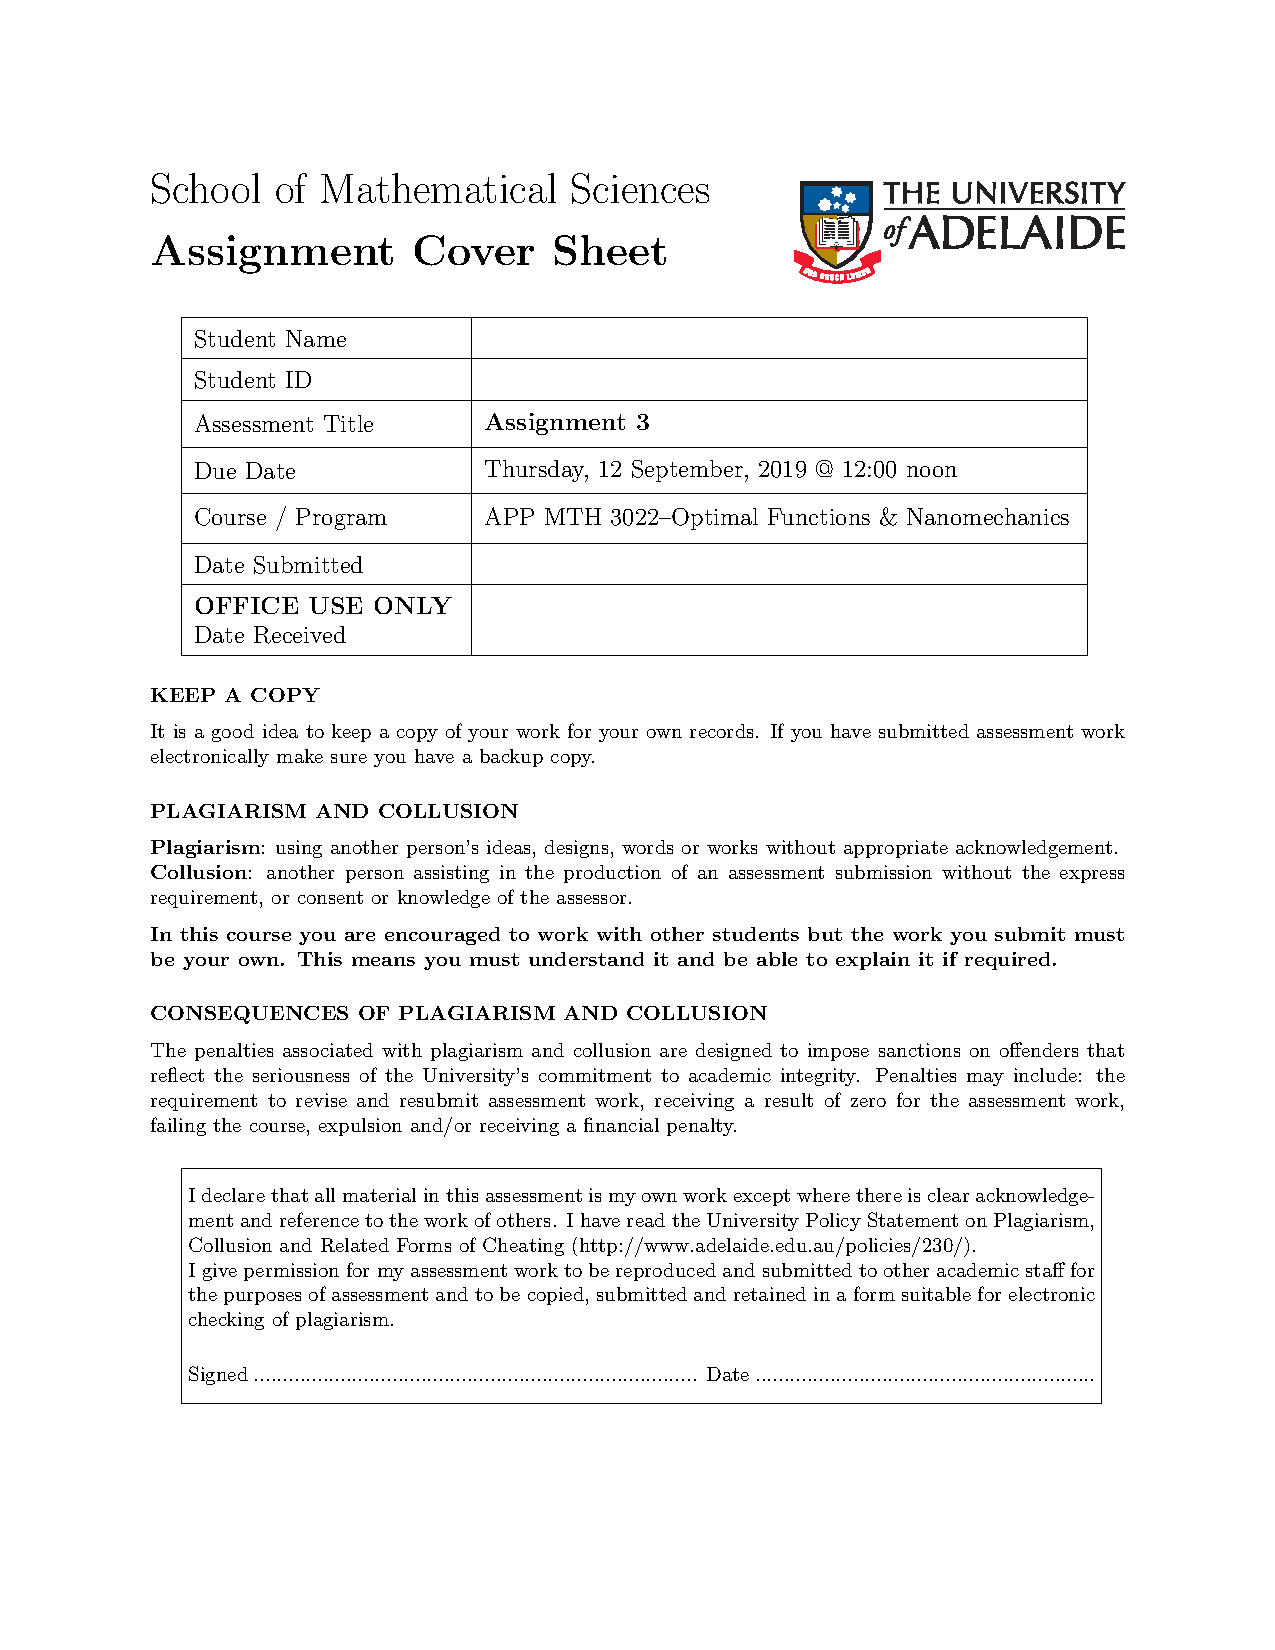
\includepdf{cover3}
\maketitle

\begin{enumerate}
%1
\item Find the form of extremals to the following
\begin{enumerate}
	%1a
	\item  
	\[F\{y(x),z(x)\} = \int_{x_0}^{x_1} (8yz - 5y^2 + y'^2 - 4z'^2) dx\]
	Let $f =  8yz - 5y^2 + y'^2 - 4z'^2 $


	The Euler-Lagrange equations are
	\begin{align*}
		\odd{}x \left(\dd f{y'}\right) - \dd fy =0 \\
		\odd{}x \left(\dd f{z'}\right) - \dd fz =0 \\
	\end{align*}
	Where
	\begin{align*}
		\dd f{y'} &= 2y', \quad \dd fy =8z - 10y\\
		\dd f{z'} &= -8z', \quad \dd fz =8y
	\end{align*} 

	Plugging into EL
	\begin{align*}
		2y'' - 8z + 10y = 0\\
		-8z'' - 8y = 0
	\end{align*}
	We get
	\[y = -z''\]
	Use this in the first equation to get a fourth order ODE
	\[-2 z^{(4)} - 8z - 10z'' = 0 \implies z^{(4)} + 4z + 5 z''\]
	Using the characteristic equation:
	\begin{align*}
		\lambda^{4}  + 5\lambda^{2} + 4 = 0\\
		\mu^2 + 5\mu + 4 = 0\\
		(\mu +1)(\mu + 4) = 0\\
		\implies \mu = -1, \quad \mu = -4\\
		\implies \lambda = \pm i, \quad \lambda = \pm 2i
	\end{align*}
	Hence the $z$ solution is
	\[\boxed{z(x) = c_1\sin(x) + c_2\cos(x) + c_3 \sin(2x) + c_4 \cos(2x) }\]
	And hence
	\[\boxed{y(x) = -z'' = c_1\sin(x) + c_2\cos(x) + 4c_3\sin(2x) + 4c_4\cos(2x)}\]
	
	Giving the extremal
	\begin{align*}
		F &= \int_{x_0}^{x_1} (8yz - 5y^2 + y'^2 - 4z'^2) dx
	\end{align*}

	%1b
	\item 
	\[F\{\vec q\} = \int_{t_0}^{t_1} \left(\dot{q_1} q_2 + \dot{q_2} q_3 + q_1 \dot{q_3} - \dot{q_1}^2\right) dt\]
	Where $\dot{q_i} := \odd{q_i}{t} $

	EL is the set of equations
	\[\odd{}t\left( \dd f{\dot{q_i}}\right) - \dd f{q_i} =0\]

	\begin{align*}
		\dd f{\dot{q_1}} = q_2 - 2\dot{q_1} ,\quad \dd f{q_1} = \dot{q_3}\\
		\dd f{\dot{q_2}} = q_3 ,\quad \dd f{q_2} = \dot{q_1}\\
		\dd f{\dot{q_3}} = q_1 ,\quad \dd f{q_3} = \dot{q_2}\\
	\end{align*}

	So the EL equations are:
	\begin{align*}
		\dot{q_2} - 2\ddot{q_1} - \dot{q_3} = 0\\
		\dot{q_3} - \dot{q_1} =0 \\
		\dot{q_1} - \dot{q_2} = 0
	\end{align*}
	\begin{align}
		\dot{q_2} - 2\ddot{q_1} - \dot{q_3} = 0\\
		\dot{q_1} = \dot{q_3} \\
		\dot{q_1} = \dot{q_2} 		
	\end{align}
	Using $(2),(3)$ shows that 
	\[\dot{q_1} = \dot{q_2} = \dot{q_3}\]
	And hence $(1)$ gives
	\[ - 2\ddot{q_1} = 0 \implies q_1 = at + c_1\]
	And hence 
	\begin{align*}
		q_1 &= at + c_1\\
		q_2 &= at + c_2\\
		q_3 &= at + c_3
	\end{align*}

	Hence the extremal has form
	\begin{align*}
		 F &= \int_{t_0}^{t_1} \left(\dot{q_1} q_2 + \dot{q_2} q_3 + q_1 \dot{q_3} - \dot{q_1}^2\right) dt
	\end{align*}
\end{enumerate}

%2
\item Find the extremal to
\[F\{y\} = \int_0^1 \left(y''^2 - 360 x^2 y\right) dx\]
Subject to $y(0) = 0, y'(0) = 1, y(1) =1,$ and $y'(1) = 5/2$

$f =y''^2 - 360 x^2 y $
\begin{align*}
	\dd f{y''} = 2y'',\quad \dd f{y'} = 0 ,\quad \dd fy = -360 x^2\\
\end{align*}
EL gives
\begin{align*}
	0 &=\dd fy - \odd{}x \left(\dd f{y'}\right) + \oddn{}x2 \left(\dd f{y''}\right)\\
	&=	-360x^2 + 2y^{(4)}\\
	y^{(4)} &= 180x^2\\
	y &= a + bx + cx^2 + dx^3 + \frac{x^6}{2}
\end{align*}

BCs
\begin{align*}
	y(0) &= 0 \implies a = 0\\
	y'(0) &= 1 \implies b=1\\
	y(1) &= 1 \implies 1 + c + d + \frac12 = 1\\
	y'(1) &= 5/2 \implies 1 + 2c + 3d + 5/2 = 5/2
\end{align*}
\begin{align*}
	c + d = - \frac12\\
	c + \frac32 d = -\frac12
\end{align*}
Hence $d = 0$ and $ c = -\frac12$
Hence
\[\boxed { y(x) = x - \frac12 x^2 + \frac{x^6}{2} }\]

%3
\item 
\begin{enumerate}
	%3a
	\item Consider the integral definition of the beta function
	
	\begin{equation}
		B(x,y) = \int_0^1 t^{x-1} (1-t)^{y-1} dt	
		\label{betafunc}
	\end{equation}
	\begin{enumerate}
	 	%3ai
	 	\item Write an integral expression for $B(z-\frac12, z+ \frac12)$
	 	\begin{align*}
	 		B(z-\frac12,z+\frac12) &= \int_0^1 t^{z-\frac12-1} (1-t)^{z+\frac12-1} dt\\
	 		&=\int_0^1 t^{z-\frac32} (1-t)^{z-\frac12} dt\\
	 	\end{align*}
	 	%3aii 
	 	\item Substitute $2t = 1+s$ into it (take care on the limits)
	 	
	 	$t = 0$ gives $s = -1$ and $t = 1$ gives $s =1$, and $dt = 1/2 ds$
	 	\begin{align*}
	 		B(z-\frac12,z+\frac12)&=\int_0^1 t^{z-\frac32} (1-t)^{z-\frac12} dt\\
	 		&= \frac12 \int_{-1}^{1} \left(\frac{1+s}{2}\right)^{z-\frac32} \left(1 - \left(\frac{1+s}{2}\right)\right)^{z-\frac12} ds\\
	 		&= \frac12 \int_{-1}^{1} \left(\frac{1+s}{2}\right)^{z-\frac32} \left(\frac{1-s}{2}\right)^{z-\frac12} ds\\
	 		&= 2^{-1}\int_{-1}^{1} \left(1+s\right)^{z-\frac32} 2^{\frac32 - z} \left(1-s\right)^{z-\frac12} 2^{\frac12 - z} ds\\
	 		&= 2^{1-2z} \int_{-1}^{1} \left(1+s\right)^{z-\frac32} \left(1-s\right)^{z-\frac12} ds\\
	 		&= 2^{1-2z} \int_{-1}^{1} \left(1-s^2\right)^z  \left(1+s\right)^{-\frac32}\left(1-s\right)^{-\frac12} ds
	 	\end{align*}
	 	%3aiii 
	 	\item Decompose into even and odd parts in $s$

	 	To decompose a function $f(x)$ into even and odd parts:
	 	\[f(x) = f_e(x) + f_o(x) = \frac{f(x) + f(-x)}{2} + \frac{f(x) - f(-x)}{2}\]
	 	So
	 	\[f(s) = (1-s^2)^z (1+s)^{-3/2} (1-s)^{-1/2}\]
	 	\begin{align*}
	 		f_e(s) &= \frac{(1-s^2)^z (1+s)^{-3/2} (1-s)^{-1/2}}{2 } + \frac{(1-s^2)^z (1-s)^{-3/2} (1+s)^{-1/2}}{2}\\
	 		f_o(s) &= \frac{(1-s^2)^z (1+s)^{-3/2} (1-s)^{-1/2}}{2 } - \frac{(1-s^2)^z (1-s)^{-3/2} (1+s)^{-1/2}}{2}\\
	 	\end{align*}
	 	So we have
	 	\begin{align*}
	 		&=  2^{1-2z} \int_{-1}^{1} \left(1-s^2\right)^z  \left(1+s\right)^{-\frac32}\left(1-s\right)^{-\frac12} ds\\
	 		&=2^{1-2z} \left(\int_{-1}^{1} f_e(s) ds + \int_{-1}^1 f_o(s) ds\right)\\
	 		&=2^{1-2z} \left(\int_{-1}^{1} \frac{(1-s^2)^z (1+s)^{-3/2} (1-s)^{-1/2}}{2 } + \frac{(1-s^2)^z (1-s)^{-3/2} (1+s)^{-1/2}}{2} ds\right. 
	 		\\&+ \left. \int_{-1}^1 \frac{(1-s^2)^z (1+s)^{-3/2} (1-s)^{-1/2}}{2 } - \frac{(1-s^2)^z (1-s)^{-3/2} (1+s)^{-1/2}}{2} ds\right)\\
	 	\end{align*}


	 	%3aiv
	 	\item Use parity to half the integration ranges in each integral. \textit{Hint} bisect the interval and sub $\sigma = -s$ into the negative interval

	 	Is this just to show that integrals over symmetric endpoints are
	 	\begin{itemize}
	 		\item Double one side for even;
	 		\item equal to zero for odd?
	 	\end{itemize}

	 	Even interval, $F_e$
	 	\begin{align*}
	 		F_e(z) &= \int_{-1}^{1} \frac{(1-s^2)^z (1+s)^{-3/2} (1-s)^{-1/2}}{2 } + \frac{(1-s^2)^z (1-s)^{-3/2} (1+s)^{-1/2}}{2} ds\\\\
	 		&= \int_{0}^{1} \frac{(1-s^2)^z (1+s)^{-3/2} (1-s)^{-1/2}}{2 } + \frac{(1-s^2)^z (1-s)^{-3/2} (1+s)^{-1/2}}{2} ds\\
	 		&-\int_{1}^0 \frac{(1- \sigma^2)^z (1- \sigma)^{-3/2} (1+ \sigma)^{-1/2}}{2 } + \frac{(1- \sigma^2)^z (1+ \sigma)^{-3/2} (1- \sigma)^{-1/2}}{2} d \sigma\\\\
	 		&= \int_{0}^{1} \frac{(1-s^2)^z (1+s)^{-3/2} (1-s)^{-1/2}}{2 } + \frac{(1-s^2)^z (1-s)^{-3/2} (1+s)^{-1/2}}{2} ds\\
	 		&+\int_{0}^1 \frac{(1- \sigma^2)^z (1- \sigma)^{-3/2} (1+ \sigma)^{-1/2}}{2 } + \frac{(1- \sigma^2)^z (1+ \sigma)^{-3/2} (1- \sigma)^{-1/2}}{2} d \sigma\\\\
	 		&= \int_0^1 (1-s^2)^z (1+s)^{-3/2} (1-s)^{-1/2} + (1-s^2)^z (1-s)^{-3/2} (1+s)^{-1/2} ds
	 	\end{align*}
	 	
	 	\begin{align*}
	 		F_o(z) &= \int_{-1}^{1} \frac{(1-s^2)^z (1+s)^{-3/2} (1-s)^{-1/2}}{2 } - \frac{(1-s^2)^z (1-s)^{-3/2} (1+s)^{-1/2}}{2} ds\\\\
	 		&= \int_{0}^{1} \frac{(1-s^2)^z (1+s)^{-3/2} (1-s)^{-1/2}}{2 } + \frac{(1-s^2)^z (1-s)^{-3/2} (1+s)^{-1/2}}{2} ds\\
	 		&+\int_{1}^0 \frac{(1- \sigma^2)^z (1- \sigma)^{-3/2} (1+ \sigma)^{-1/2}}{2 } + \frac{(1- \sigma^2)^z (1+ \sigma)^{-3/2} (1- \sigma)^{-1/2}}{2} d \sigma\\\\
	 		&= \int_{0}^{1} \frac{(1-s^2)^z (1+s)^{-3/2} (1-s)^{-1/2}}{2 } + \frac{(1-s^2)^z (1-s)^{-3/2} (1+s)^{-1/2}}{2} ds\\
	 		&-\int_{0}^1 \frac{(1- \sigma^2)^z (1- \sigma)^{-3/2} (1+ \sigma)^{-1/2}}{2 } + \frac{(1- \sigma^2)^z (1+ \sigma)^{-3/2} (1- \sigma)^{-1/2}}{2} d \sigma\\\\
	 		&= 0
	 	\end{align*}
	 	Hence the full integral is
	 	\[2^{1-2z}(F_e + F_o) = 2^{1-2z}\int_0^1 (1-s^2)^z (1+s)^{-3/2} (1-s)^{-1/2} + (1-s^2)^z (1-s)^{-3/2} (1+s)^{-1/2} ds\]
	 	% %3av 
	 	\item Use $\tau = s^2$ to get the form from eqn~\ref{betafunc} 


	 	$\tau = s^2$ gives $ds = \frac1{2\sqrt{\tau}} d \tau = 2^{-1} \tau^{-1/2} d \tau$ and bounds stay the same 
	 	\begin{align*}
	 		&= 2^{1-2z}\int_0^1 (1-s^2)^z (1+s)^{-3/2} (1-s)^{-1/2} + (1-s^2)^z (1-s)^{-3/2} (1+s)^{-1/2} ds\\
	 		&= 2^{1-2z}\int_0^1\left((1-s) +(1+s)\right) (1-s^2)^z (1-s)^{-3/2} (1+s)^{-3/2} ds***\\
	 		&= 2^{1-2z}\int_0^1 2(1-s^2)^z (1-s)^{-3/2} (1+s)^{-3/2} ds\\
	 		&= 2^{1-2z}\int_0^1 2(1-s^2)^z ((1-s)(1+s))^{-3/2} ds\\
	 		&= 2^{1-2z}\int_0^1 2(1-s^2)^z (1 - s^2)^{-3/2} ds\\
	 		&= 2^{1-2z}\int_0^1 (1- \tau)^{z-3/2} \tau^{-1/2}d \tau\\
	 		&= 2^{1-2z}\int_0^1 \tau^{-1/2} (1- \tau)^{z-3/2} d \tau\\
	 		&= 2^{1-2z} B(1/2,z-1/2)
	 	\end{align*}

	 	$***$ putting the two parts even, I have multiplied the left part by $(1-s)^{2/2} (1-s)^{-2/2}$ and the right part by $(1+s)^{2/2} (1+s)^{-2/2}$, i.e. multiplying by $1$.
	 	
	 	%3avi 
	 	\item Using all the previous parts, and the relationship between the beta and gamma functions, derive
	 	\[\Gamma(2z) = 2^{2z-1} \pi^{-1/2} \Gamma(z) \Gamma(z+1/2)\]
	 	We have the beta/gamma relationship:
	 	\[B(x,y) = \frac{\Gamma(x) \Gamma(y)}{\Gamma(x+y)}\]
	 	\begin{align*}
	 		 B(z-\frac12,z + \frac12) &= 2^{1-2z} B(\frac12,z-\frac12)\\
	 		 \frac{\Gamma(z-\frac12)\Gamma(z+\frac12)}{\Gamma(z-\frac12 + z + \frac12)} &=2^{1-2z} \frac{\Gamma(\frac12) \Gamma(z-\frac12)}{\Gamma(z)}\\
	 		 \frac{\Gamma(z+\frac12)}{\Gamma(2z)} &=2^{1-2z} \frac{\pi^{-1/2}}{\Gamma(z)}\\
	 		\implies \Gamma(2z) &= 2^{2z-1} \pi^{-1/2} \Gamma(z) \Gamma(z+1/2)
	 	\end{align*}
	 \end{enumerate}
	
	%3b
	\item  From the integral definitions given in class, show
	\[K(k) = \frac{\pi}{2} F(1/2,1/2;1;k^2)\]
	Note that, using Euler's integral formula
	\begin{align*}
		F(a,b;c;z) &= \frac{\Gamma(c)}{\Gamma(b)\Gamma(c-b)} \int_0^1 t^{b-1} (1-t)^{c-b-1} (1-tz)^{-a} dt\\
		F(1/2,1/2;1;k^2) &= \frac{\Gamma(1)}{\Gamma(1/2) \Gamma(1/2)} \int_0^1 t^{-1/2}(1-t)^{-1/2} (1-tk^2)^{-1/2} dt\\
		&= \frac{1}{\pi} \int_0^1 t^{-1/2}(1-t)^{-1/2} (1-tk^2)^{-1/2} dt\\
	\end{align*}
	Sub $t = \sin^2 \vartheta$, $dt = 2\sin\cos\vartheta d\theta$, and $t=1$ gives $\vartheta = \pi/2$
	\begin{align*}
		F(1/2,1/2;1;k^2) &= \frac{1}{\pi} \int_0^1 t^{-1/2}(1-t)^{-1/2} (1-tk^2)^{-1/2} dt\\
		&=\frac1{\pi} \int_0^{\pi/2} \frac{1}{\sin\vartheta} \frac{1}{\sqrt{1-\sin^2\vartheta}} \frac{1}{\sqrt{1-k^2\sin^2\vartheta}}2\sin\cos\vartheta d\vartheta\\
		&= \frac2{\pi} \int_0^{\pi/2}  \frac{1}{\cos\vartheta} \frac{1}{\sqrt{1-k^2\sin^2\vartheta}}\cos\vartheta d\vartheta\\
		&= \frac2{\pi} \int_0^{\pi/2}\frac{1}{\sqrt{1-k^2\sin^2\vartheta}}d\vartheta\\
	\end{align*}
	Where $F(\varphi,k)$ denotes the elliptic integral of the first kind, we get:
	\begin{align*}
		K(k) &= F(\pi/2,k)\\
		&= \int_0^{\pi/2} \frac{d\vartheta}{\sqrt{1-k^2\sin^2\vartheta}}\\
		&= \frac{\pi}{2}\frac2{\pi} \int_0^{\pi/2}\frac{1}{\sqrt{1-k^2\sin^2\vartheta}}d\vartheta\\
		&= \frac{\pi}{2} F\left(1/2,1/2;1;k^2\right)
	\end{align*}
	As required

\end{enumerate}
\end{enumerate}

\end{document}